\documentclass[border=10pt]{standalone}

\usepackage{tikz}
\usepackage{tikzsymbols}
\usetikzlibrary{calc,patterns,shapes.geometric}

\def\centerarc[#1](#2)(#3:#4:#5){\draw[#1] ($(#2)+({#5*cos(#3)},{#5*sin(#3)})$) arc (#3:#4:#5);}

\begin{document}
	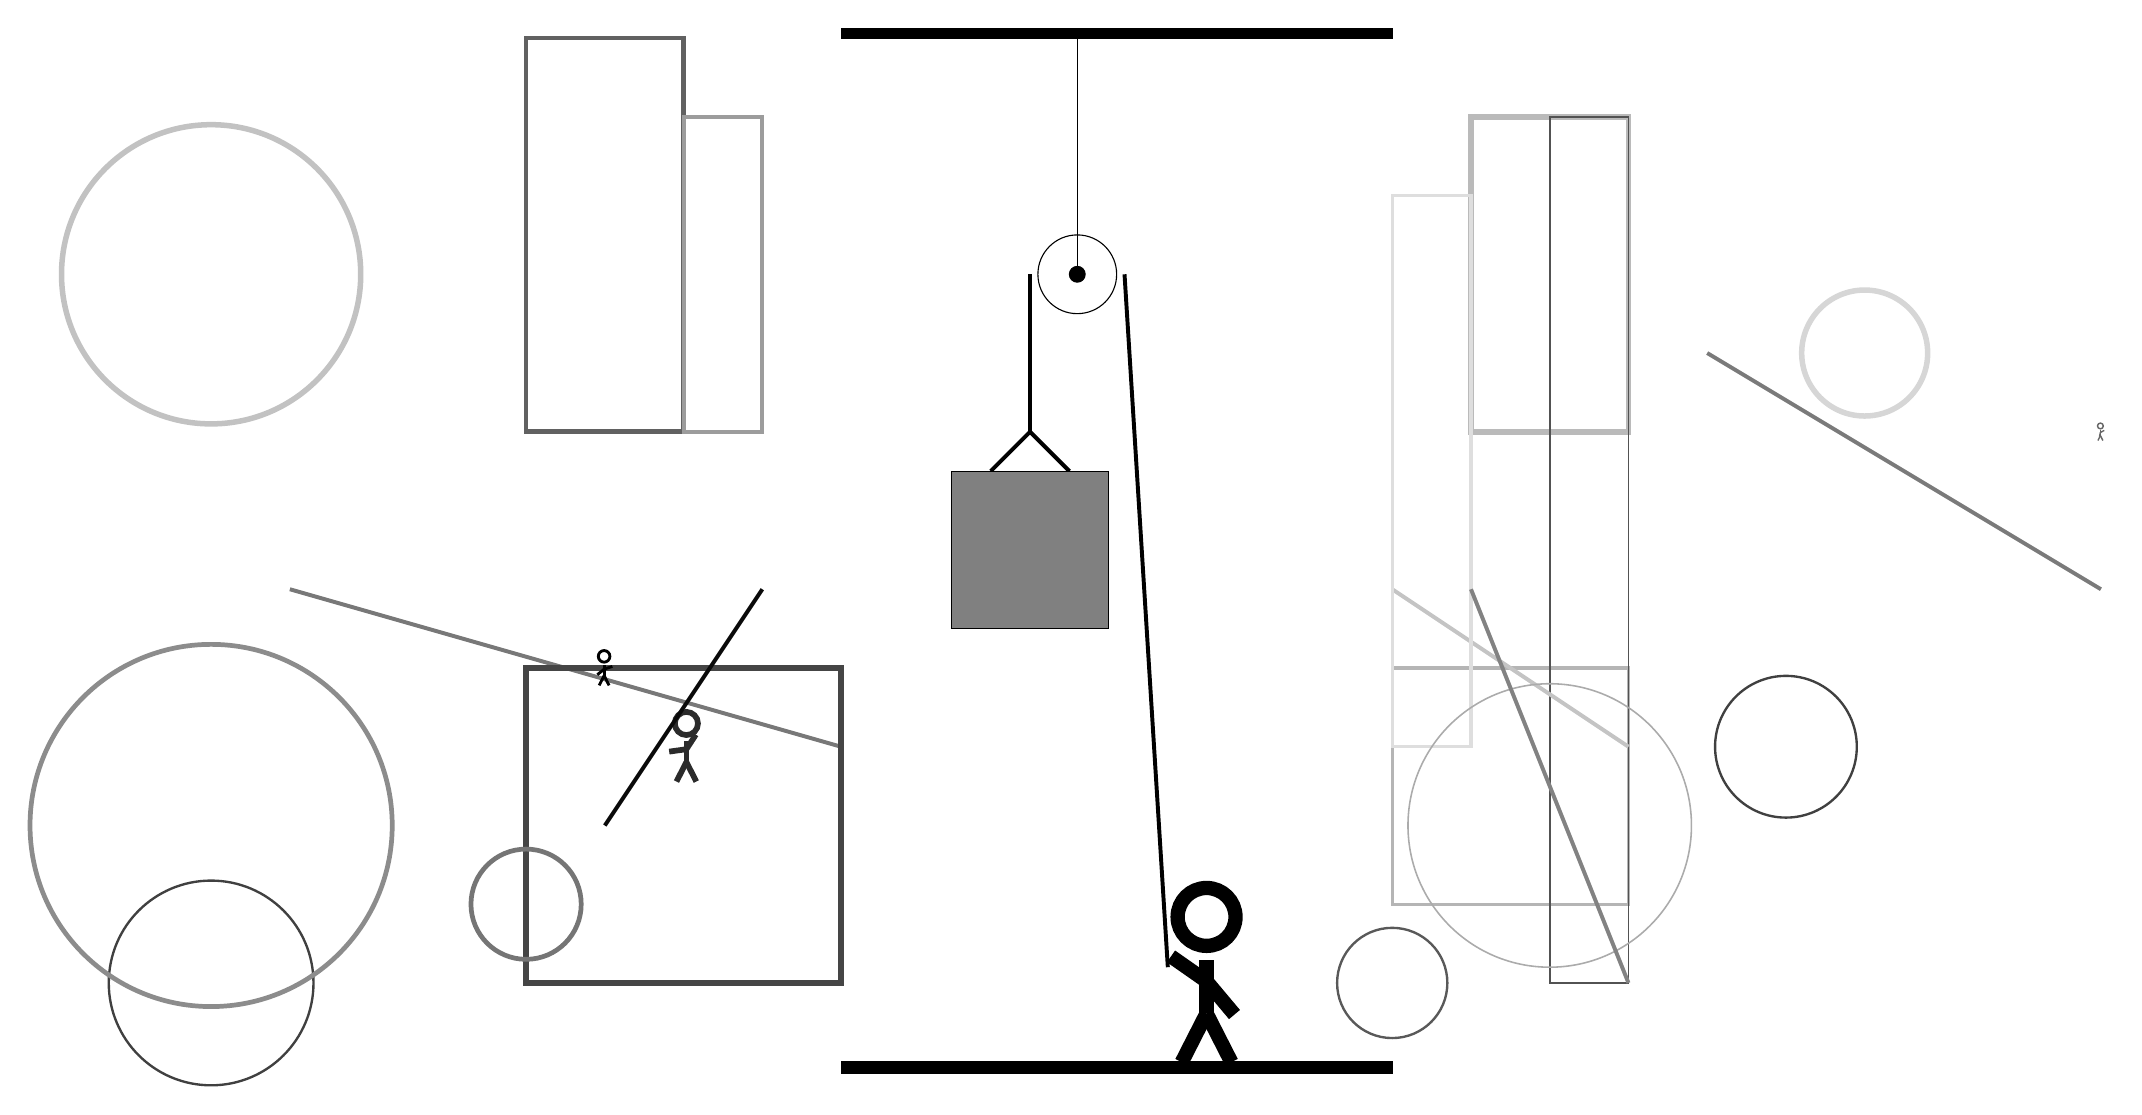
\begin{tikzpicture}
		%%%%% START %%%%%
		
		\draw[fill=black] (-2, 10) rectangle (5, 10.125);
		
		\draw[line width=0.4mm, color=black!29] (5, 2) rectangle (8, -1);
		
		\draw[line width=0.7mm, color=black!27] (6, 5) rectangle (8, 9);
		\draw[line width=0.6mm, color=black!62] (-4, 5) rectangle (-6, 10);
		\node[line width=0.2mm, color=black!83] at (-4, 1) {\Strichmaxerl[4][8][57]};
		\draw[line width=0.2mm, color=black!68] (7, 9) rectangle (8, -2);
		
		\draw[line width=0.5mm, color=black!23](5, 3) -- (8, 1);
		\node[line width=0.3mm, color=black!60] at (14, 5) {\Strichmaxerl[1][78][27]};
		\draw[line width=0.5mm, color=black!53](-2, 1) -- (-9, 3);
		\draw[line width=0.4mm, color=black!13] (6, 1) rectangle (5, 8);
		\draw [line width=0.2mm, color=black!33](7, 0) circle (1.8);
		\draw[line width=0.7mm, color=black!73] (-2, 2) rectangle (-6, -2);
		\draw [line width=0.7mm, color=black!16](11, 6) circle (0.8);
		\draw[line width=0.2mm, color=black!39] (-2, -3) rectangle (-2, -3);
		
		\draw [line width=0.3mm, color=black!75](-10, -2) circle (1.3);
		\draw [line width=0.3mm, color=black!65](5, -2) circle (0.7);
		\draw[line width=0.5mm, color=black!49](6, 3) -- (8, -2);
		\draw [line width=0.6mm, color=black!45](-10, 0) circle (2.3);
		
		\node[line width=0.7mm, color=black!100] at (-5, 2) {\Strichmaxerl[2][39][19]};
		\draw[line width=0.5mm, color=black!39] (-3, 5) rectangle (-4, 9);
		
		\draw [line width=0.7mm, color=black!24](-10, 7) circle (1.9);
		\draw [line width=0.3mm, color=black!75](10, 1) circle (0.9);
		
		\draw[line width=0.5mm, color=black!96](-3, 3) -- (-5, 0);
		\draw[line width=0.5mm, color=black!52](9, 6) -- (14, 3);
		\draw [line width=0.6mm, color=black!54](-6, -1) circle (0.7);
		
		\draw (1, 7) circle (0.5);
		\draw[fill=black] (1, 7) circle (0.1);
		\draw (1, 10) -- (1, 7);
		
		\draw[line width=0.5mm] (-0.1, 4.5) -- (0.4, 5.0) -- (0.9, 4.5);
		\draw[fill=black!50] (-0.6, 4.5) rectangle (1.4, 2.5);
		
		\draw[line width=0.5mm] (0.4, 7) -- (0.4, 5.0);
		\centerarc[line width=0.5mm](1, 7)(0:180:0.6);
		\draw[line width=0.5mm](1.6, 7) -- (2.15, -1.8);
		
		\node at (2.6, -1.9) {\Strichmaxerl[10][-35][-50]};
		
		\draw[fill=black] (-2, -3) rectangle (5, -3.15);
		
		%%%%% END %%%%%
	\end{tikzpicture}
\end{document}